\documentclass[a4paper,12pt]{article}

%% Language and font encodings
\usepackage[italian]{babel}
\usepackage[utf8x]{inputenc}
\usepackage[T1]{fontenc}

%% Sets page size and margins
\usepackage[a4paper,top=2cm,bottom=2cm,left=3cm,right=3cm,marginparwidth=1.75cm]{geometry}

%% Useful packages
\usepackage{graphicx}
\usepackage{bigstrut}
\usepackage{hyperref}
\usepackage[figurename=Figura]{caption}
\usepackage[tablename=Tabella]{caption}
\hypersetup{colorlinks=true, urlcolor=blue, linkcolor=black}
\title{Alberi di decisione con dati mancanti}
\author{*}

\begin{document}
\maketitle

\section{Introduzione}
Lo scopo di questo elaborato è quello di valutare le accuratezze ottenute dall'algoritmo di apprendimento per alberi di
decisione al variare della percentuale dei dati mancanti nel dataset.

\
\begin{figure}[h]
    \centering
    \captionsetup{justification=centering,margin=1cm}
    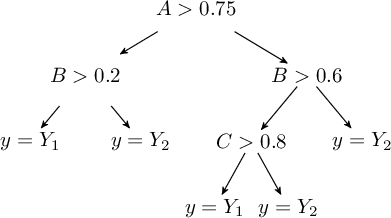
\includegraphics[width=0.6\textwidth]{./fig_decisiontree}
    \vspace*{5mm}
    \caption{Un esempio di albero di decisione. [\textit{ce.unipr.it}]}
    \label{fig:dec}
\end{figure}

\subsection{Alberi di decisione}

Nell’ambito del \textit{Machine Learning} un metodo semplice ed efficace per risolvere problemi di classificazione è quello di utilizzare gli alberi di decisione.
\newline

 Un albero di decisione, costruito a partire da un insieme di dati iniziali (\textbf{dataset}), è un albero in cui ogni nodo interno è associato ad una particolare “domanda” su una certa caratteristica dei dati. Da questo nodo escono tanti archi quanti sono i possibili valori che la caratteristica può assumere, fino a raggiungere le foglie che indicano la categoria associata alla decisione.
 \newline

 Lo scopo è quello di allenare questo albero su alcuni esempi di dati (\textit{training set}) in modo da poter classificare altri dati non precedentemente visionati (\textit{test set}) con un certo livello di confidenza.
\newline

Un problema comune con gli alberi di decisione è che spesso si adattano fin troppo bene ad alcune caratteristiche specifiche solo del \textit{training set}, e questo porta ad un calo delle prestazioni sul \textit{test set}. Si parla in questo caso di \textit{\textbf{overfitting}}.

Esistono comunque diverse tecniche per prevenire l'\textit{overfitting}: una di queste è l'utilizzo della \textit{cross validation} (vedi sezione \ref{ssec:cval}).

\subsection{Gestione dei valori mancanti} \label{ssec:val}
L'algoritmo standard per l'apprendimento tramite alberi di decisione non gestisce i casi in cui alcuni esempi
siano privi di qualche attributo. 
\newline

Una strategia per la gestione di questi casi è quella di assegnare all'attributo mancante
il valore più comune che esso assume rispetto a tutti gli altri esempi che raggiungono il nodo.
\newline

Un'altra strategia, più complessa, è quella di far finta che l'esempio abbia \textit{tutti} i possibili valori
dell'attributo, pesando però ognuno di questi in base alla sua frequenza negli esempi che raggiungono il nodo. 
In questo caso l'algoritmo di classificazione dovrebbe quindi seguire tutti i rami uscenti dal nodo per cui manca il valore
dell'attributo e moltiplicare i pesi lungo ogni cammino.
\newline

Ai fini di questo elaborato è stato scelto di utilizzare la prima strategia.

\section{Esperimento}
L'esperimento si può dividere in due fasi.
\newline

Nella prima fase è stato implementato in Python l’algoritmo di apprendimento per alberi di decisione descritto
in classe, ed è stata aggiunta la strategia per gestire valori mancanti, come riportato nella sezione
\ref{ssec:val}.
\newline

Nella seconda fase è stato applicato l'algoritmo a problemi di classificazione su tre datasets scelti
da \href{http://archive.ics.uci.edu/ml/index.php}{UCI Machine Learning Repository}, calcolandone l'accuratezza con \textit{10-fold cross-validation} dopo aver rimosso,
rispettivamente, lo 0\%, il 10\%, il 20\% e il 50\% dei dati.
\newline

Le accuratezze sono state poi inserite in un grafico, riportato nella sezione \ref{ssec:ris}.

\section{Implementazione}
Il progetto è stato sviluppato con Python versione 3.6 e richiede l'installazione della libreria
\textit{matplotlib} per la generazione di grafici in 2d.

\subsection{Alberi di decisione}
La struttura di un albero di decisione (nodo, rami, foglia) è implementata nei file 
\textit{\textbf{decision\_leaf.py}} e \textit{\textbf{decision\_fork.py}}. La classe \textit{DecisionLeaf} ha come unico attributo il risultato della predizione. La classe \textit{DecisionFork}, invece, contiene l'attributo da testare e un dizionario che rappresenta i vari rami, uno per ogni possibile valore dell'attributo stesso.
\newline

L'algoritmo standard per l'apprendimento tramite alberi di decisione, implementato in forma ricorsiva, si trova invece nel
file \textit{\textbf{dt\_learner.py}} il quale attinge anche da altre funzioni di aiuto che si trovano in \textit{\textbf{utils.py}}.

\subsection{Cross validation e gestione di attributi mancanti} \label{ssec:cval}
Per testare l'accuratezza dell'algoritmo e per evitare \textit{overfitting} viene richiesta la tecnica di \textit{\textbf{k-fold cross-validation}}, implementata nel file 
\textit{\textbf{cross\_validation.py}}.

 Essa consiste nella suddivisione del dataset in k parti uguali e, ad ogni passo, la k-esima parte del dataset si considera come \textit{test set}, mentre la restante parte costituisce il \textit{training set}. Si allena quindi il modello sul \textit{training set} e si cerca di predire il restante gruppo con le conoscenze acquisite. L'accuratezza è il rapporto tra il numero di predizioni corrette e il numero di predizioni totali.
 \newline

Per una maggiore precisione questo procedimento può essere ripetuto più volte (è il parametro \textit{trials} della funzione \textit{cross\_validation()}), ogni volta rimescolando il dataset, per poi prendere la media dei risultati come stima dell'accuratezza.
\newline

La gestione dei valori mancanti avviene nel file \textit{\textbf{missing\_values.py}}. Per prima cosa la funzione \textit{randomly\_remove\_values()} prende in ingresso un dataset e la probabilità \textit{p} di rimuovere un elemento, e restituisce un nuovo dataset (lasciando inalterato l'originale), uguale ma con gli elementi rimossi uniformemente e casualmente rispetto a \textit{p}.


La funzione \textit{handle\_missing\_values()}, invece, prende in ingresso un dataset e sostituisce tutti gli eventuali valori mancanti di un attributo con il valore più comune che assume quell'attributo rispetto agli altri esempi (vedi sezione \ref{ssec:val}).

\subsection{Dataset}
Nel file \textit{\textbf{dataset.py}} è stata fornita una implementazione della classe \textit{DataSet}. Essa contiene una lista di esempi (righe di valori di attributi) e un target (l'indice di un attributo che l'algoritmo proverà a predire).
\newline

Nella cartella \textit{./datasets/} sono presenti tre dataset, reperiti da \textit{UCI ML Repository}: \textit{car.txt, phishing.txt, nursery.txt}. Per maggiori informazioni su questi dataset si rimanda al file \textit{README.txt} all'interno della cartella.

\subsection{Test}
Nel file \textit{\textbf{tests.py}} sono stato eseguiti i seguenti esperimenti:
\newline

- Per ognuno dei tre dataset, è stata calcolata l'accuratezza con 10 trials di \textit{10-fold cross-validation}, dopo aver rimosso alcuni attributi uniformemente e casualmente con le probabilità p=[0.0, 0.1, 0.2, 0.5].
\newline

- Dopo aver quindi ottenuto quattro accuratezze per ogni dataset, i dati sono stati riportati in un grafico generato con la libreria \textit{matplotlib}. 
\newline

I risultati sono riportati di seguito.

\clearpage
\section{Risultati} \label{ssec:ris}
Di seguito sono riportati i risultati di una possibile esecuzione dei test.

\begin{center}
\vspace*{0.9cm}
\begin{tabular}{|c|c|c|c|c|}
\hline
& \textbf{0\%}\bigstrut & \textbf{10\%} & \textbf{20\%} & \textbf{50\%} \\\hline
\textbf{car.txt}\bigstrut & 93.709\% & 78.593\% & 72.1881\% & 67.3322\%\\\hline
\textbf{phishing.txt}\bigstrut & 88.3074\% & 82.114\% & 78.6847\% & 70.716\%\\\hline
\textbf{nursery.txt}\bigstrut & 98.8657\% & 81.713\% & 65.7191\% & 51.0756\%\\\hline
\end{tabular}
\captionsetup{justification=centering}
\captionof{table}{Accuratezze rilevate al variare della percentuale di dati mancanti.}
\label{tab:tab1}
\end{center}

\begin{figure}[h]
    \centering
    \vspace*{0.2cm}
    \captionsetup{justification=centering,margin=1cm}
    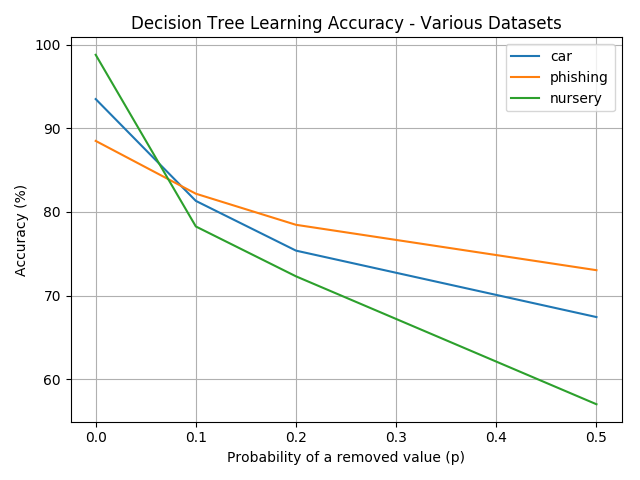
\includegraphics[width=0.93\textwidth]{./plot}
    \caption{Gli stessi dati della Tabella \ref{tab:tab1}, riportati in un grafico.}
    \label{fig:plot}
\end{figure}
\

Aldilà delle differenze tra i dataset, relative principalmente al diverso numero di esempi e/o di attributi, dal grafico si può osservare come l'andamento delle tre curve sia sostanzialmente lo stesso.
\newline

Infatti, come ci si poteva aspettare, l'accuratezza dell'algoritmo di learning risulta inversamente proporzionale al numero di dati mancanti nel dataset.  In altre parole, più ci sono dati mancanti nel dataset e più è difficile l'apprendimento, a prescindere dalla bontà del modello utilizzato.
\newline

\end{document}